$ \forall x (P(x) \lor Q(x)) \models \forall x P(x), \forall x Q(x) $ 
\begin{center}
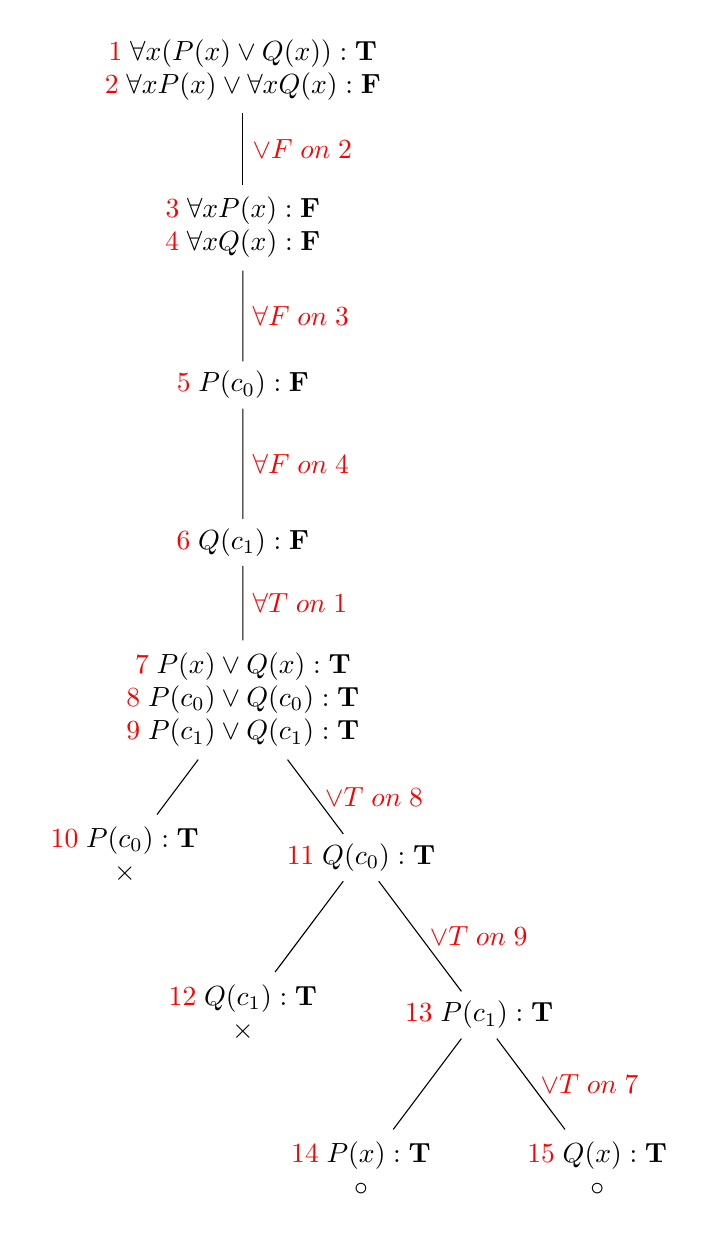
\begin{tikzpicture}

\node {$ \begin{array}{c} \textcolor{red}{1}\; \forall x (P(x) \lor Q(x)):\textbf{T} \\ \textcolor{red}{2}\; \forall x P(x) \lor \forall x Q(x):\textbf{F} \end{array} $} [sibling distance = 2cm] [level distance=20mm] 
        child {node {$ \begin{array}{c} \textcolor{red}{3}\; \forall x P(x):\textbf{F} \\ \textcolor{red}{4}\; \forall x Q(x):\textbf{F} \end{array} $} 
            child {node {$ \textcolor{red}{5}\; P(c_0):\textbf{F} $}
                child {node {$ \textcolor{red}{6}\; Q(c_1):\textbf{F} $}
                    child {node {$ \begin{array}{c} \textcolor{red}{7}\; P(x) \lor Q(x):\textbf{T} \\ \textcolor{red}{8}\; P(c_0) \lor Q(c_0):\textbf{T} \\ \textcolor{red}{9}\; P(c_1) \lor Q(c_1):\textbf{T} \end{array} $} [sibling distance = 3cm]
                        child {node {$ \begin{array}{c} \textcolor{red}{10}\; P(c_0):\textbf{T} \\ \times \end{array} $}} 
                        child {node {$ \textcolor{red}{11}\; Q(c_0):\textbf{T} $}
                            child {node {$ \begin{array}{c} \textcolor{red}{12}\; Q(c_1):\textbf{T} \\ \times \end{array} $}} 
                            child {node {$ \textcolor{red}{13}\; P(c_1):\textbf{T} $}
                                child {node {$ \begin{array}{c} \textcolor{red}{14}\; P(x):\textbf{T} \\ \circ \end{array} $}} 
                                child {node {$ \begin{array}{c} \textcolor{red}{15}\; Q(x):\textbf{T} \\ \circ \end{array} $}                            
                                    edge from parent node [right, red] {$\lor T\;on\; 7$}}
                                    edge from parent node [right, red] {$\lor T\;on\; 9$}}
                                    edge from parent node [right, red] {$\lor T\;on\; 8$}}
                                    edge from parent node [right, red] {$\forall T\;on\; 1$}}
                                    edge from parent node [right, red] {$\forall F\;on\; 4$}}
                                    edge from parent node [right, red] {$\forall F\;on\; 3$}} 
                                    edge from parent node [right, red] {$\lor F\;on\; 2$}};

\end{tikzpicture}
\end{center}

In order to determine if a predicate logic formula is satisfiable we use the tableau method. Setting the root formula equal to false allows us to investigate it. If all branches are closed it means that the formula is valid, if only some are closed it means that there are some truth assignment that make the formula true and other that make the formula false (satisfiable) and when all branches are open the formula never evaluates to true.

\begin{center}
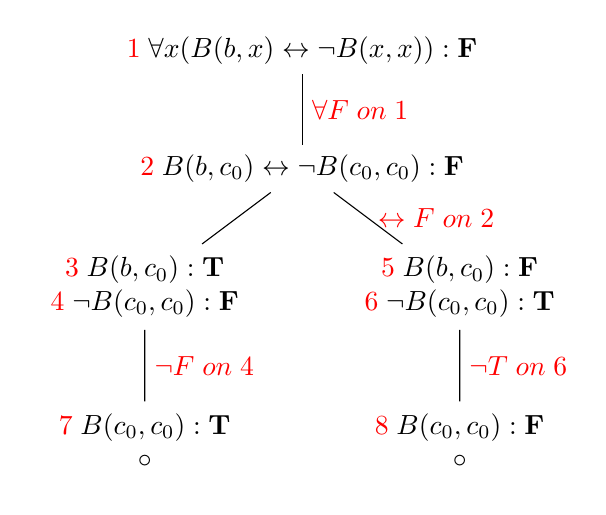
\begin{tikzpicture}

\node {$ \textcolor{red}{1}\; \forall x (B(b,x) \leftrightarrow \neg B(x,x)):\textbf{F} $} [sibling distance = 2cm] 
        child {node {$ \textcolor{red}{2}\; B(b,c_0) \leftrightarrow \neg B(c_0,c_0):\textbf{F} $} [sibling distance = 4cm] 
            child {node {$ \begin{array}{c} \textcolor{red}{3}\; B(b,c_0):\textbf{T} \\ \textcolor{red}{4}\; \neg B(c_0,c_0):\textbf{F} \end{array} $} [level distance=20mm]
                child {node {$ \begin{array}{c} \textcolor{red}{7}\; B(c_0,c_0):\textbf{T} \\ \circ \end{array} $} 
                edge from parent node [right, red] {$\neg F\;on\; 4$}}}
            child {node {$ \begin{array}{c} \textcolor{red}{5}\; B(b,c_0):\textbf{F} \\ \textcolor{red}{6}\; \neg B(c_0,c_0):\textbf{T} \end{array} $} [level distance=20mm]
                child {node {$ \begin{array}{c} \textcolor{red}{8}\; B(c_0,c_0):\textbf{F} \\ \circ \end{array} $}
                                    edge from parent node [right, red] {$\neg T\;on\; 6$}}
                                    edge from parent node [right, red] {$\leftrightarrow F\;on\; 2$}} 
                                    edge from parent node [right, red] {$\forall F\;on\; 1$}};

\end{tikzpicture}
\end{center}